%%%%%%%%%%%%%%%%%%%%%%%%%%%%%%%%%%%%%%%%%%%%%%%%%%%%%%%%%%%%%%%%%%%%%%%%%%%%%%%%
%2345678901234567890123456789012345678901234567890123456789012345678901234567890
%        1         2         3         4         5         6         7         8

\documentclass[letterpaper, 10 pt, conference]{ieeeconf}  % Comment this line out
                                                          % if you need a4paper
% * <nhatkhanh98@gmail.com> 2018-03-12T09:27:56.013Z:
%
% ^.
%\documentclass[a4paper, 10pt, conference]{ieeeconf}      % Use this line for a4
                                                          % paper

\IEEEoverridecommandlockouts                              % This command is only
                                                          % needed if you want to
                                                          % use the \thanks command
\overrideIEEEmargins
% See the \addtolength command later in the file to balance the column lengths
% on the last page of the document



% The following packages can be found on http:\\www.ctan.org
%\usepackage{graphics} % for pdf, bitmapped graphics files
%\usepackage{epsfig} % for postscript graphics files
%\usepackage{mathptmx} % assumes new font selection scheme installed
%\usepackage{times} % assumes new font selection scheme installed
\usepackage{amsmath} % assumes amsmath package installed
\usepackage{amssymb}  % assumes amsmath package installed
\usepackage{amsfonts}
\usepackage{url}
\def\UrlBreaks{\do\/\do-}
\usepackage{graphicx}
\usepackage{breakurl}
\usepackage{array}
\usepackage{multicol}
\usepackage{csquotes}
%\usepackage{hyperref}

\title{\LARGE \bf
Improving Keypoint-matching Methods for Food and Beverage \\Logo Detection and Recognition
}

\author{ \parbox{3 in}{\centering Nhat-Khanh Nguyen-Ba\\
		 Advanced Program in Computer Science\\
         University of Science\\
         Hochiminh City, Vietnam\\
         {\tt\small nbnkhanh@apcs.vn}}
         \hspace*{ 0.5 in}
         \parbox{3 in}{ \centering Thai-Bao Do\\
         Advanced Program in Computer Science\\
         University of Science\\
         Hochiminh City, Vietnam\\
         {\tt\small dtbao@apcs.vn}}
         \\
         \\
         \parbox{3 in}{ \centering Nhat-Minh Ha\\
         Advanced Program in Computer Science\\
         University of Science\\
         Hochiminh City, Vietnam\\
         {\tt\small hnminh@apcs.vn}}
         \hspace*{ 0.5 in}
         \parbox{3 in}{ \centering The-Loc Tran\\
         Advanced Program in Computer Science\\
         University of Science\\
         Hochiminh City, Vietnam\\
         {\tt\small ttloc@apcs.vn}}
}

%\author{Huibert Kwakernaak$^{1}$ and Pradeep Misra$^{2}$% <-this % stops a space
%\thanks{*This work was not supported by any organization}% <-this % stops a space
%\thanks{$^{1}$H. Kwakernaak is with Faculty of Electrical Engineering, Mathematics and Computer Science,
%        University of Twente, 7500 AE Enschede, The Netherlands
%        {\tt\small h.kwakernaak at papercept.net}}%
%\thanks{$^{2}$P. Misra is with the Department of Electrical Engineering, Wright State University,
%        Dayton, OH 45435, USA
%        {\tt\small p.misra at ieee.org}}%
%}


\begin{document}



\maketitle
\thispagestyle{empty}
\pagestyle{empty}


%%%%%%%%%%%%%%%%%%%%%%%%%%%%%%%%%%%%%%%%%%%%%%%%%%%%%%%%%%%%%%%%%%%%%%%%%%%%%%%%
\begin{abstract}

Food and beverage industry has developed rapidly since in Vietnam, its user penetration rate was at 4.50\% in 2017. Conducting customer experience research, which is the important work to develop offline-to-online commerce, is one of the main demand of food and beverage companies. Logo detection and recognition acts as a simple, natural but potential method since logos are the identity of the brands. The authors propose an improvement of Flann-based Matcher that inherits from uniform sampling method and saliency detection. By applying this improvement, companies can detect their logos in images from social networks like Facebook, Instagram, etc. and classify them based on the logos’ locations to obtain the customers’ opinions. Finally, the authors experimentally show that the accuracy increases 5.00\% compared to original method on a subset of Flickr27 dataset combining with images collected from social networks.
\end{abstract}
\begin{keywords}
object detection, object recognition, feature extraction, Flann-based matcher, uniform sampling
\end{keywords}

%%%%%%%%%%%%%%%%%%%%%%%%%%%%%%%%%%%%%%%%%%%%%%%%%%%%%%%%%%%%%%%%%%%%%%%%%%%%%%%%
\section{INTRODUCTION}
There is a growing demand for evaluating products of companies based on customers' experience. Companies desire to understand customers' behavior to deliver products that they need. In order to make a right decision for marketing revenue to gather interest for brands, many methods have been proposed. \par
%tach doan nay ra, thay Triet keu (Khanh)
One of the approaches is applying text-based social listening and sentiment analysis through captions and comments of customers. The problem is that photos are replacing text at an accelerating rate. According to the report of social media by Social Media Examiner in 2016, \enquote{74\% of social media marketers use visual assets in their social media marketing}, the most of all types\cite{social-media-report} .\par
The iconic property of a brand is its logo. Therefore, companies invest more in logo detection and recognition tools to achieve digital marketing opportunity through visual analytics and visual listening\cite{5reasons}. This approach gives companies a chance to keep track of the coverage of their brands. Moreover, through this approach and social listening, companies can also have the information of customers' opinions of their brand and their opponents' brands, which is a huge competitive element.\par
With rapidly evolving social media, photos are everywhere and this is highly potential for marketing since logo is one of the fastest ways to raise the exposure of a brand. It is important that our target is focusing more on pictures with product logos in high saliency regions, one of them is the center area to pictures. As our work is to develop a logo recognizing solution for capturing the spread of brand identity, those pictures have a higher chance with people's comments being related to the brand. \par
In fact, more than 250 billion photos have been uploaded to Facebook\cite{facebook1}, and 350 million photos per day, which means 4,000 photos per second in 2018\cite{facebook1}. On January 2016, Buzzsumo, a company that has analyzed over 1 billion posts on Facebook from 30 millions brand pages, shows that posts with images, one of the 6 types of post, have the engagement  (total numbers of likes, shares and comments) 5 times more than the others\cite{facebook3}. For Instagram, since 2010, more than 40 billion have been uploaded so far, and 95 million photos per day, or about 1,100 photos per second on average\cite{instagram}. With a huge number of photos, the automatic logo detection and recognition based on images is inevitable. Moreover, these tremendous figures motivate the authors to develop a method that can incorporate with real-time applications. Therefore, keypoint-matching is one of the traditional but efficient approach of logo detection and recognition.\par
To conduct experiments, the authors evaluate the methods using Flickr27\cite{619} as dataset in the beginning. Since some images in Flickr27 have logos not located at the center area of the images and not related to food and beverage, the removal of unrelated images is necessary. Therefore, the dataset which is used in the experiment is a collection of the subset dataset Flickr27 and images on the Internet to meet the requirement in terms of quantity in each experimented logo.\par
Initially, the input is a query image, which is the sample logo, and a train image. Both are detected to find local interest points (or keypoints), which are distinguished parts of an image. Then descriptors, which are the numerical vectors representation of the keypoints, are computed, followed by the matching process. The authors describe the previous work on local feature extraction and matching algorithm in section II. However, the problems of false matches and having few features to match are the main obstacles. The authors investigate how the above problems degrade the performance of traditional methods such as SIFT\cite{sift} and ORB\cite{orb}. From the results, the authors observe improvements through sequence of proposed methods, discussed in details in section III, based on uniform sampling that helps increasing the number of good matches. This improvement gives a remarkable result that is discussed in section IV. Unfortunately, the problem still remains. The authors draw interesting conclusions and necessary works in the future in section V.\par
%................%
\section{RELATED WORK}
The algorithms used to locate the keypoints are called \textit{detectors}. They are classified into two types: \textit{corner detector} and \textit{blob detector}. The algorithms used to describe the keypoints are called \textit{descriptors}. Similar to detectors, descriptors are classified into two types: \textit{binary descriptor} and \textit{spectra descriptor}\cite{tonghop}. Concretely, binary descriptor uses the difference between pairs of pixel to compute binary values in a vector, which proves its efficiency in computing, storing, and matching using Hamming distance. In contrast, spectra descriptor uses more complex computations and requires larger memory. Spectra may be referred as histograms of local gradient orientations, light intensities, etc.\cite{tonghop}.\par
Subsection A-E are about common detectors and descriptors. Subsection F is about Brute-Force Matcher. Subsection G is about the FLANN library, which is the basis of the traditional feature matching method.
\subsection{SIFT - Blob detector and Spectra descriptor}
To extract distinctive invariant features from pictures that help solving matching problems of object recognition in disruption conditions, David G. Lowe proposed SIFT\cite{sift} keypoints detector and descriptor. This algorithm has four basic steps: estimating scale-space extreme detection using a different-of-Gaussian function, keypoint localization that based on measures of their stability, a keypoint orientation assignment based on local image gradient directions, and computing descriptor for each keypoint based on local image gradients. Due to the highly distinction of the feature, a single feature can correctly matched with high probability in large database of features using fast nearest-neighbor algorithm. He applies a cascade filtering approach and by this approach, the cost of extracting these features is minimized and large number of features are generated. In keypoint-matching problem, to prevent false matches, they show experimentally by calculating the probability that a match is correct by taking the ratio of distance from the closest neighbor to the distance of the second closest. But for being a 128-vector, the SIFT descriptor is quite slow to compute and match\cite{brief}. \par
\subsection{SURF - Blob detector and Spectra descriptor}
%SURF
A more popular feature extraction proposed by Herbert Bay et al. in 2008 is SURF (Speeded Up Robust Features)\cite{surf}. This algorithm based on a basic approximation of Hessian blob detector to get the keypoints, and the computation time is reduced due to the reliance on integral images. SIFT builds the Gaussian pyramid which downscales the image octave through octave, while SURF takes advantages of integral image to upscale the Gaussian masks instead of changing the size of the image. For this reason, SURF is shown to be remarkably faster than SIFT. Another difference is in orientation assignment: SIFT involves histograms of gradient computations, whereas in SURF, wavelet responses are used for this stage and feature description stage. The descriptors are obtained by the wavelet responses, which are taken and represented from each subregion in a selected neighborhood around the keypoint.  \par
\subsection{FAST - Corner detector}
%FAST
Another type of feature that is widely used is FAST (Features from Accelerated Segment Test), proposed by Edware Rosten and Tom Drummond in 2006\cite{fast}. It is an appealing choice for keypoint detector because of its efficiency and provision of corner keypoints. It can be explained like this: for each pixel in the image, consider a circle of sixteen pixels around it. A pixel is marked as a corner if there exists a set of a particular number $n$ of pixels in the above circle which is brighter or darker than the considered pixel plus or minus a threshold. Unlike SIFT and SURF, FAST does not have an orientation operator. The main drawback of FAST is\: the order of the mentioned sixteen pixels and the case $n<12$ affect the speed of the algorithm.\par
\subsection{BRIEF - Binary descriptor}
%BRIEF
A large number of feature descriptors has been proposed, one of the popular descriptors is BRIEF (Binary Robust Independent Elementary Features) by Michael Calonder et al. in 2010\cite{brief}. The descriptor uses binary tests to present an smoothed image patch as a binary string. Each bit can be obtained by comparing the intensities of pairs of points based on Hamming distance, and on modern CPUs, this process can be done significantly fast. One drawback of BRIEF is its sensitiveness to in-plane rotation and scale changes. \par
%ORB
\subsection{ORB - Corner detector and Binary descriptor}
In addition, in 2011, Ethan Rublee et al. proposed ORB (Oriented FAST and Rotated BRIEF)\cite{orb} which has been proven efficient alternative to SIFT. ORB is a modified combination of FAST detector and BRIEF descriptors. It not only has expected enhanced processing time to be 100 times faster with no less performance comparing to SIFT but it also solves computational problems of SIFT with the same matching technique. Moreover, the method is rotation invariant, resistant to noise and free from restriction. The efficiency of ORB is demonstrated through experiments on attributes similar to SIFT as well as testing on patch tracking application. The results shows the importance of variance under orientation to its execution and advantage over SIFT.
\subsection{Brute-Force Matcher}
Brute-Force Matcher is created based on a brute force algorithm\cite{opencv_library}. Brute-Force Matcher takes the descriptor of one feature in the set of features in the first images. This descriptor is used to match all other features in the second set of features in the second image. The result returns in two way according to the function in library. One way is that it returns the closest match feature and the another way returns the best k-matches features in the second image corresponded to the descriptor. 
\subsection{FLANN library}
Combining with SIFT\cite{sift},  David G. Lowe and Marius Muja proposed "Fast Approximate Nearest Neighbors with Automatic Algorithm Configuration" with the goal is to determine the fastest approximate nearest-neighbor algorithm\cite{flann}. Concretely, the input is any given dataset respective to desired degree of precision while the output is the best algorithm (since the algorithm depends on the datasets) with parameter values. The new algorithm applies priority search on hierarchical k-means trees instead of branch-and-bound, which is shown to reduce tree construction time and have best performance on many datasets. In other datasets, they use multiple randomized kd-trees. \par
\section{PROPOSED METHODS BASED ON \\UNIFORM SAMPLING}
\subsection{Overview}
\begin{center}
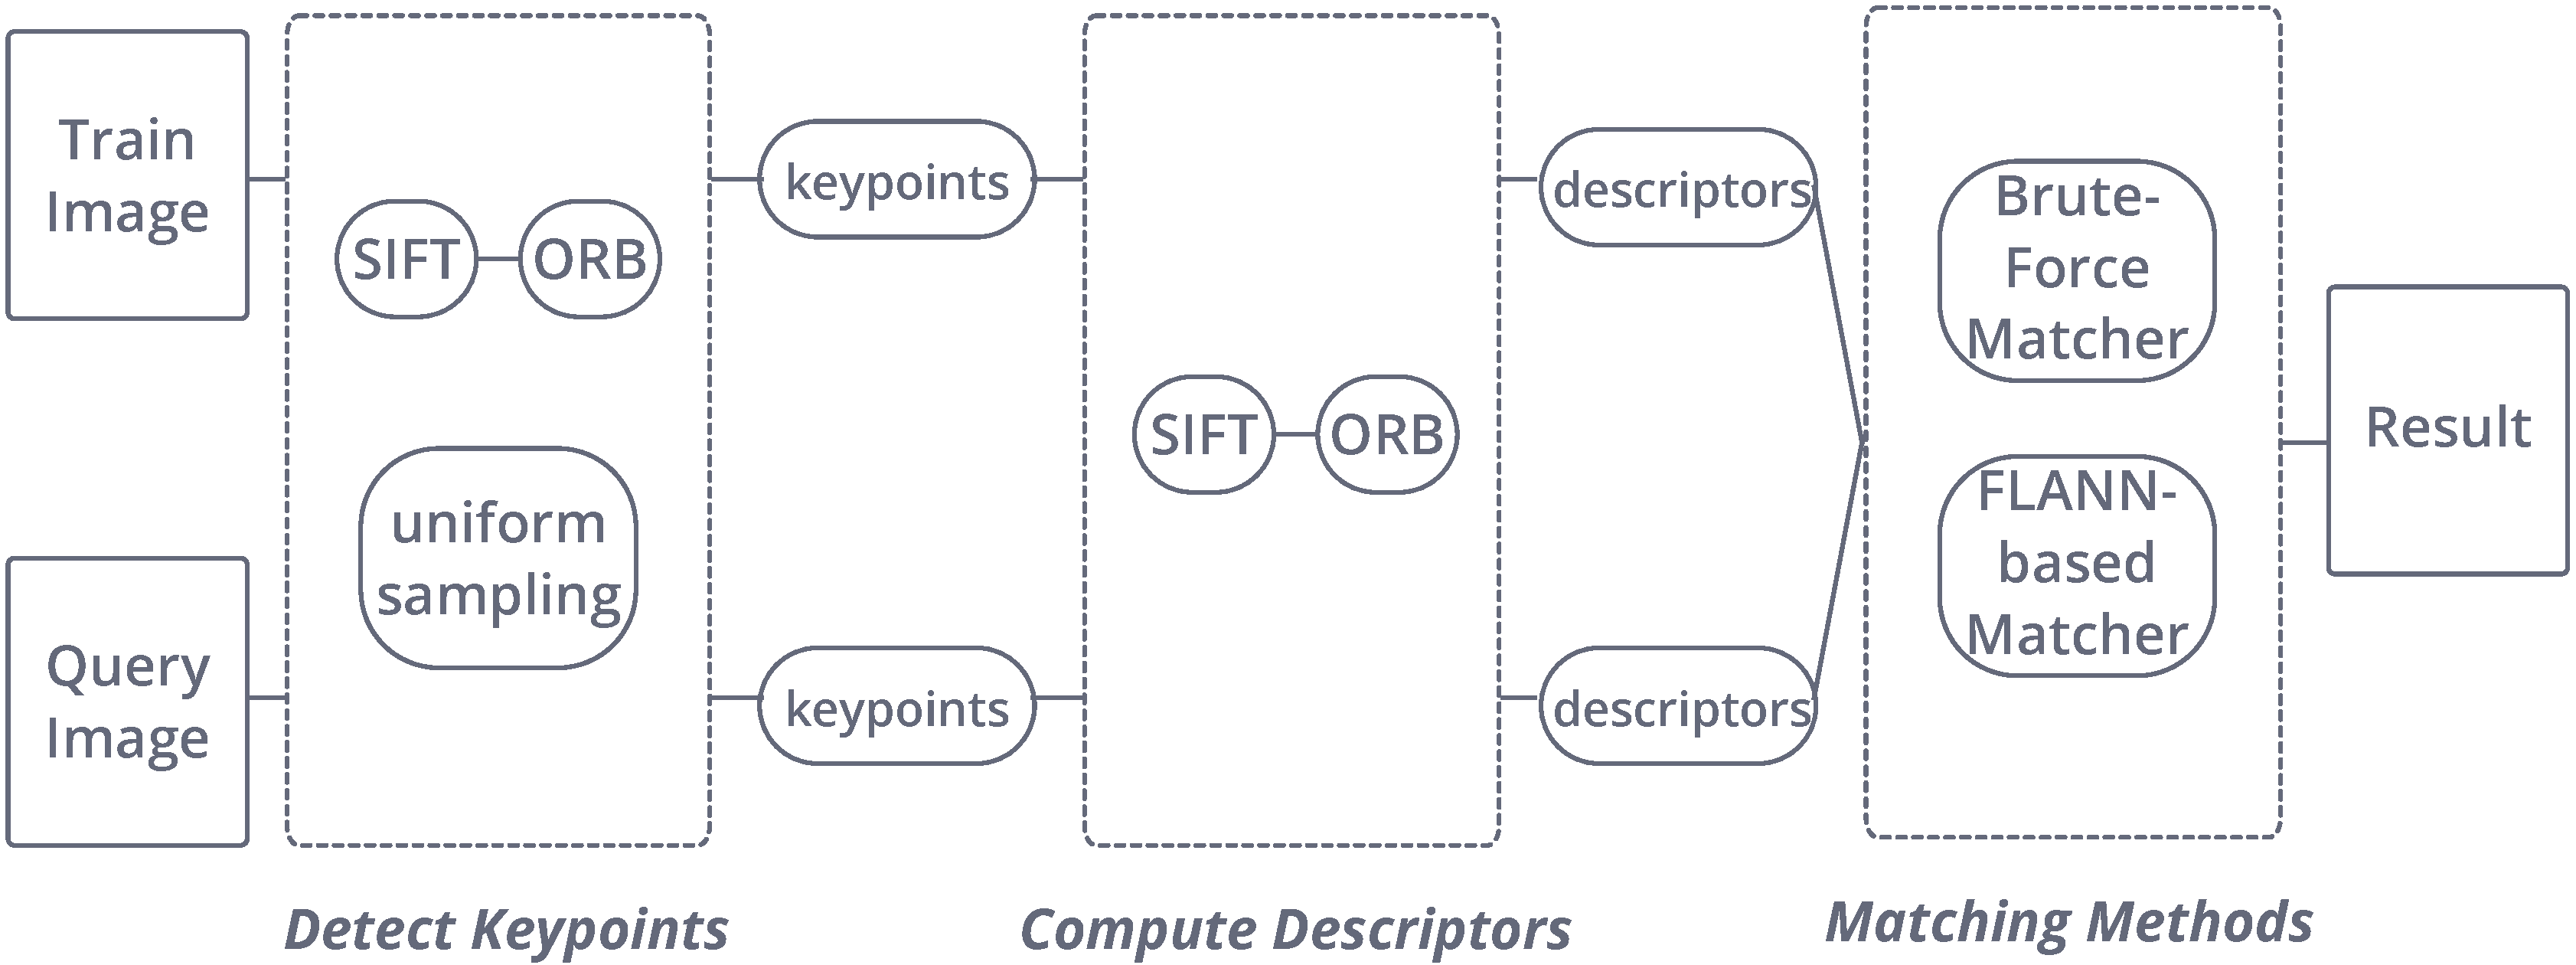
\includegraphics[width=0.5\textwidth]{quytrinhv.pdf} \\
\textbf{Figure 1. Overview of the process} \textit{}
\end{center}
\par
In this section, we describe our evaluation method on different keypoint-matching methods. The process consists of comparing different combinations of traditional keypoint-matching methods with common keypoint detectors and descriptors, followed by uniform sampling with keypoints distributed over the entire logo and on the logo edges. We compare these methods by measuring their average running time per image and getting the accuracy based on number of good matches manually. The process is illustrated in Figure 1.\par
At first, we combine Brute-force Matcher method with SIFT\cite{sift} and ORB\cite{orb}, because they are common and efficient keypoints detectors and descriptors. In most scenarios, ORB has the fastest operating speed while SIFT has highest performance. The same thing is done for Flann-based Matcher\cite{flann}, so in total there are four combinations. The ratio test proposed by David G. Lowe is applied to identify good matches\cite{sift}. But these combinations are expected to have low performance on sample logos that have few features to be detected, so an improvement is needed. For this reason, we propose a modification: instead of using detectors to locate the interesting features, we apply uniform sampling to generate our own keypoints, then use the best of above combinations to compute the descriptions and perform the matching. Observe that random keypoints usually scatter on the regions with similar features, we also propose a way to make these keypoints concentrate on the edges instead.
\subsection{Proposed method}
\subsubsection{Generating keypoints with uniform sampling method}
The goal is to deal with logos that have few features. Our approach is to "force" the keypoints to be distributed randomly. However, because we generate our own keypoints, the size of the keypoints must be considered. So by observing the common sizes of keypoints through the experiments in part A, we choose to generate keypoints with radius 5. Moreover, based on the shape of sample logos, we divide the distribution into two types: rectangle distribution for square-shaped logos and disk distribution for circular logos. For rectangle distribution, keypoints are generated randomly along the width and height of the shape. For disk distribution, it is more complex. On circular logo with radius $R$, to avoid the center-biased distribution, the transformation \[x = \sqrt{r}\cos(\theta)\] \[y = \sqrt{r}\sin(\theta)\] is applied, with $r \in [0, R^2]$ and $\theta \in [0,2\pi]$\cite{disk}. For the test image of size $a \times b$, applying saliency detection\cite{saliency}, we only distribute in the area bounded by $0.25a$ to $0.75a$ and $0.25b$ to $0.75b$, which accounts for half the image. We generate for about 200 keypoints on query image, and the number of keypoints distributed on the train image is the number of keypoints distributed on query image times the ratio between half of the area of the train image and query image. Then the combination with the best performance in part A is applied to compute the descriptors of the generated keypoints and perform the matching. Since distributing randomly over the entire logo usually results in keypoints having similar features, distributing on the edges has a more promising outcome.
\subsubsection{Conditions for a pixel to lie on the edges}
\begin{center}
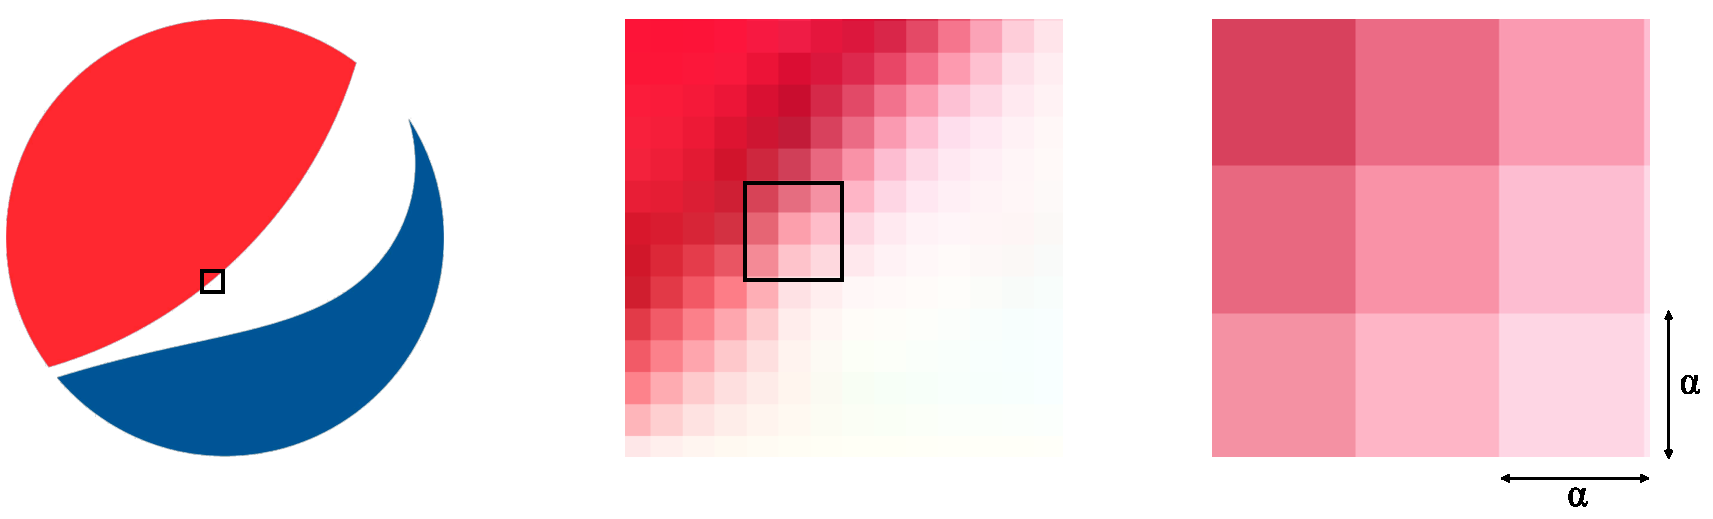
\includegraphics[width=0.5\textwidth]{minhhoaVA.pdf} \\
\textbf{Figure 2. Illustration of the proposed edge-detection method} \textit{For this illustration, $\alpha = 1$ pixel}
\end{center}
\par
This section we describe the method of determining whether a random-generated point is potentially on the edges of a logo, which is illustrated in Figure 2. An image is treated as a 2D-array in which elements are pixels with three color attributes: Red(R), Green(G), and Blue(B). The algorithm takes three parameters: $\alpha$, $\beta$, and $\gamma$. For a pixel $P(x,y)$, we consider eight direction points which are equidistant relative to P: $(x - \alpha, y + \alpha)$, $(x - \alpha, y - \alpha)$, $(x - \alpha, y)$, $(x + \alpha, y + \alpha)$, $(x + \alpha, y - \alpha)$, $(x + \alpha, y)$, $(x, y + \alpha)$, $(x, y - \alpha)$. The color-difference value of the pixel and each of its corresponding eight direction points is calculated by the L1 distance:
\[dist(X,Y) = |X[R] - Y[R]| + |X[G] - Y[G]| + |X[B] - Y[B]|\]
where $dist(X,Y)$ is the color-difference value between point $X$ and point $Y$, $X[R]$ is the red attribute of point $X$, $X[G]$ is the green attribute of point $X$, and $X[B]$ is the blue attribute of point $X$, so as point $Y$. If $dist(X,Y) \leq \gamma$, we mark that direction point as a "good" one, then we increase the counting variable. After running over eight direction points, if the counting variable is smaller than $\beta$, the considered pixel scatters on the edge of the logo with a high probability. The parameter $\beta$ is set to 4 or 5 would be a reasonable choice, because the idea behind this method is that edges are usually the boundaries of two regions with different colors.  \par 
We apply the above algorithm into the original method in part B by sequentially keeping one of the three parameters fixed, varying the others two parameters and observing the behaviors. However when the algorithm is applied to uniform sampling, the running time is prolonged because when a single keypoint is generated, we have to check whether that keypoint lies on edges. If the conditions are not met, the keypoint is discarded and the program keeps running until the desired number of keypoints is distributed.
%..............%
\section{EXPERIMENTS}
\begin{center}
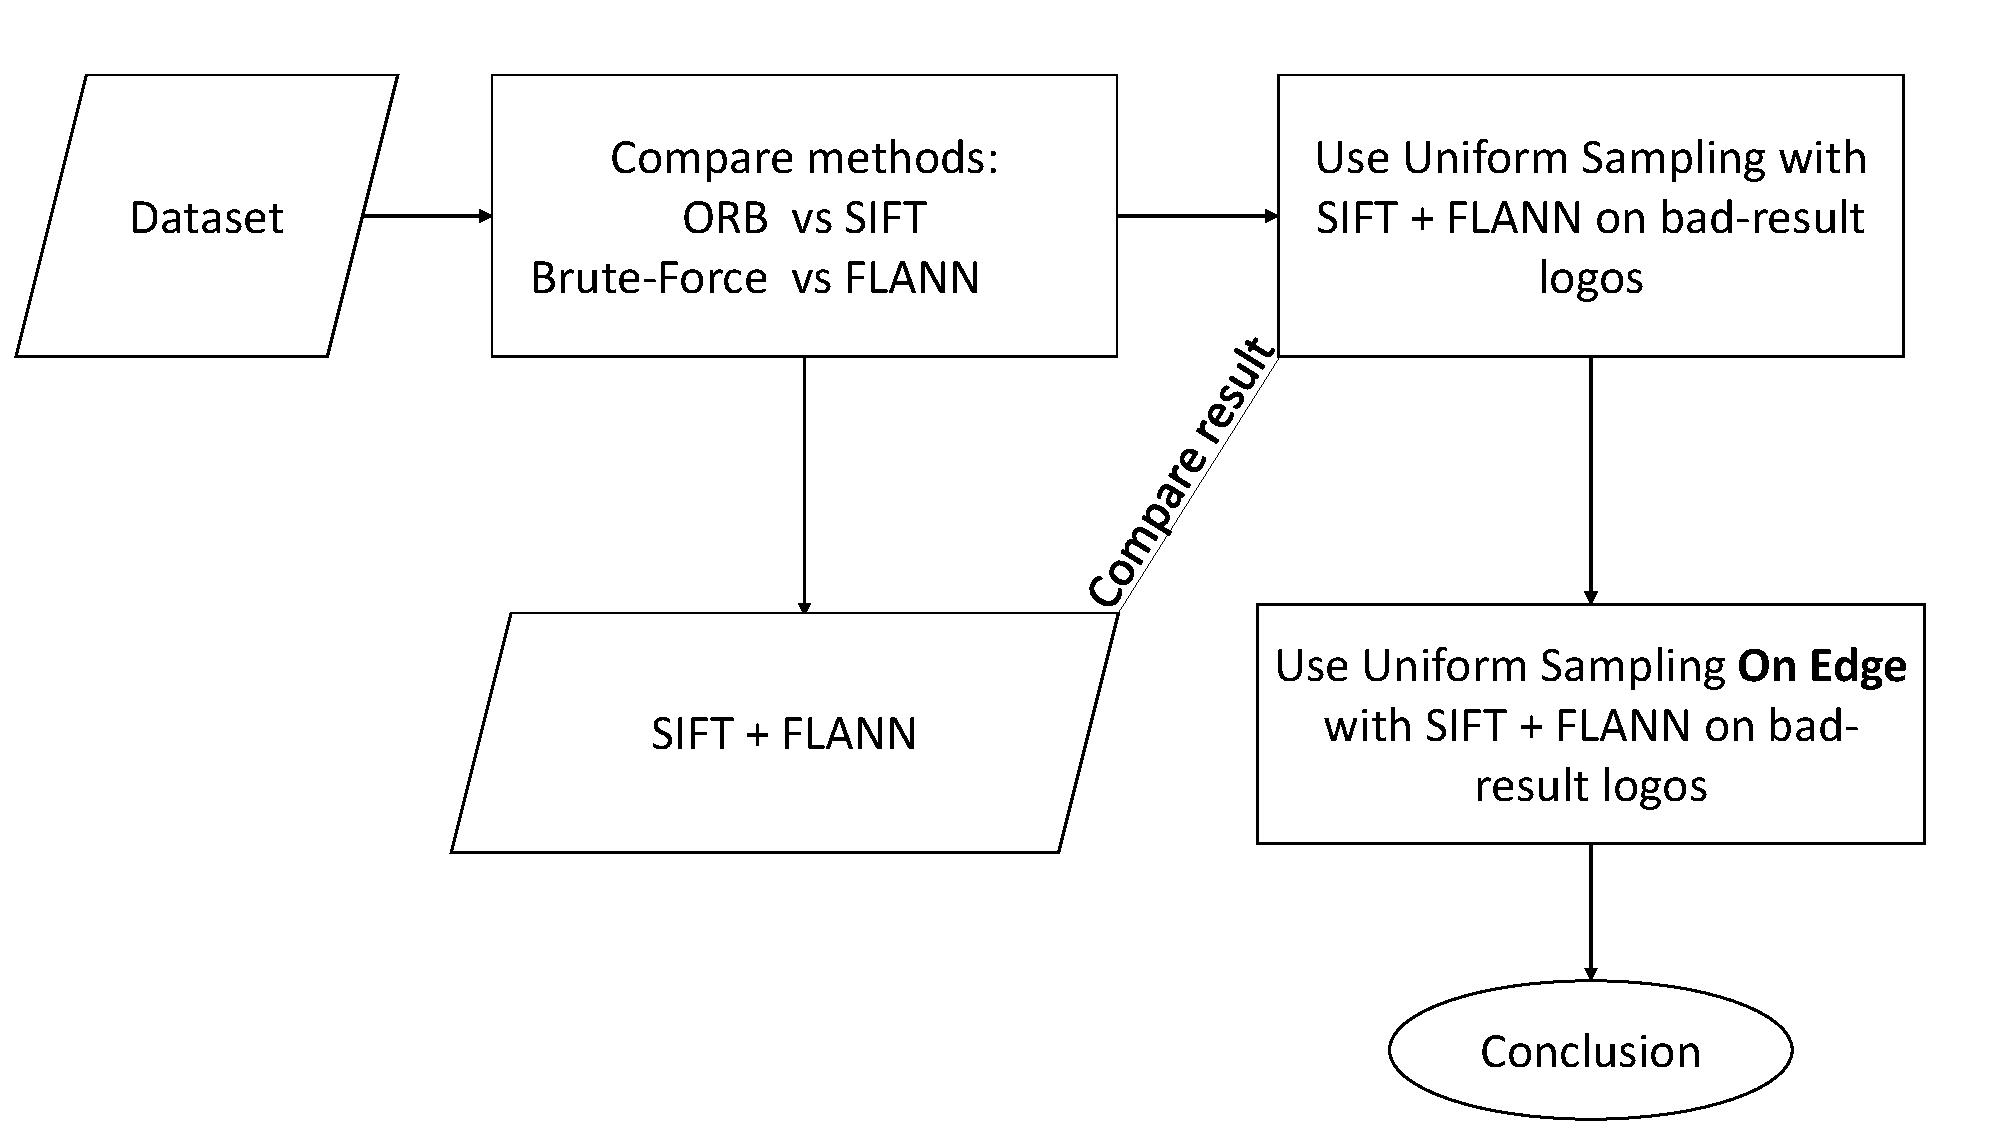
\includegraphics[width=0.5\textwidth]{Presentation1.pdf} \\
\textbf{Figure 3. Overview of the steps}
\end{center}
\par
Figure 3 shows our created dataset taken for comparing methods stage. With two keypoints detectors and descriptors: SIFT and ORB, along with two matching methods: Brute-Force Matcher and FLANN, we conduct four combinations stemmed from them to discover the best among those. Then, we apply uniform sampling method and its result is compared with the best combination which is mentioned earlier. Finally, conclusion has been made after several improvements.\par
\subsection{Dataset}
\par
\begin{center}
\begin{tabular}{|l|c|}
\hline
Logos & Quantity\\ \hline
Vinamilk & 15\\ \hline
McDonald & 20\\ \hline
Pepsi & 17\\ \hline
Heineken & 30\\ \hline
Sprite & 26\\ \hline
Coca-cola & 31\\ \hline
Starbucks & 20\\ \hline
Baskin Robbins & 21 \\ \hline
\textbf{Total} & \textbf{180} \\ \hline
\end{tabular}
\end{center}
\begin{center}
\textbf{Table 1. Dataset from eight chosen food and beverage brands}
\end{center}
\par
To evaluate the accuracy and performance of our proposed method, three following steps are carried. Before going into details about the experiments, we provide general information about our datasets. In total, there are 180 images distributed in 8 brands. Each brand contains from 15 to 31 images (Table 1). Since the target is to focus on logo in the center area of the images, we create a subset from Flickr27 dataset and collect images from Instagram due to the lack of suitable images. Moreover, we conduct the experiments on Microsoft Visual Studio on Windows environment and use Matplotlib library to visualize the matching results. The code was executed on an Intel(R) Core(TM) i7-7500U 2.70GHz (4 CPUs) processor.\par
\subsection{Compare accuracy and running time of four traditional combinations}
\begin{center}
\begin{tabular}{|l|c|}
\hline
Method & Average running time\\ \hline
SIFT-FLANN & 0.38s\\ \hline
SIFT-Brute Force & 0.39s \\ \hline
ORB-FLANN & 0.06s\\ \hline
ORB-Brute Force & 0.05s\\ \hline
\end{tabular}
\\
\end{center}
\begin{center}
\textbf{Table 2. Average running time per image of the four combinations}
\end{center}
\par
%co xoa bot 1 cau, cai y ket hop SIFT ORB FLANN lap lai nhieu qua (khanh)
\begin{figure*}
\centering
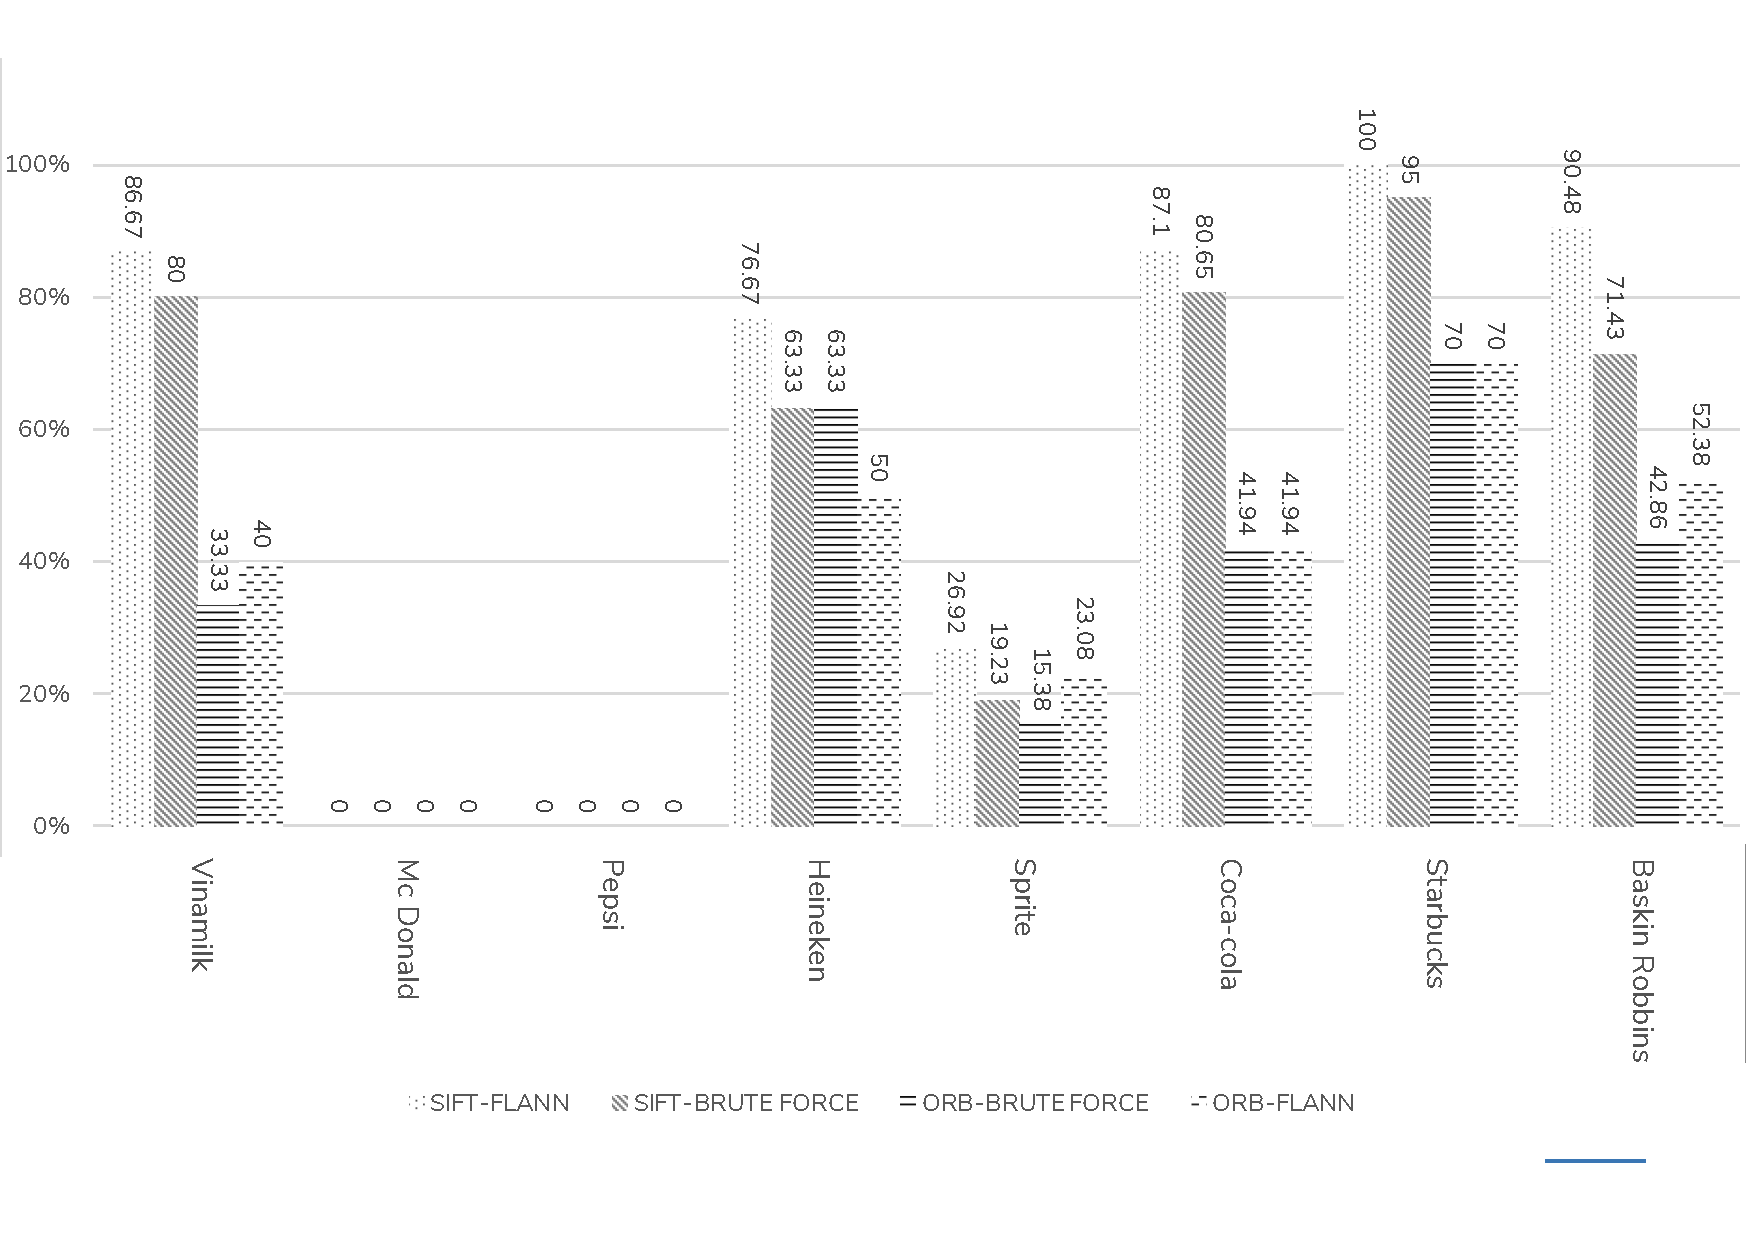
\includegraphics[width=15cm, height=8cm]{compareaccuracy.pdf}
\\
\textbf{Figure 4. Accuracy of the four combinations}
\end{figure*}
As mentioned in section III, to choose the best combination for logo detection and recognition, we conduct four experiments respective to four combinations. Figure 4 below shows the accuracy of four methods: ORB with Brute-Force Matcher, SIFT with Brute-Force Matcher, ORB with FLANN, and SIFT with FLANN. Overall, ORB-Brute Force gives the worst result (6 out of 8 logos have the accuracy below 50.00\%) while SIFT-FLANN has the highest accuracy in each logo. Pepsi and McDonald logos give undesired results 0.00\% in accuracy since few keypoints are detected. Moreover, logos of Vinamilk, Heineken, Coca-cola, Starbucks, and Baskin-Robbins return results larger than 75.00\% since these logos are more complex so that more keypoints are detected. The experiments also reveal that, when the features detected in the train image are similar to those in sample logo, the chance of false matchings increases.
%vai cho xai tu ko dung, t fix lai (khanh)


\par
Table 2 shows the average running time of each image of the two SIFT combinations and the two ORB combinations, respectively. Among four combinations, ORB-Brute-Force has the fastest running time and SIFT-FLANN has the slowest one. Moreover, in general, combinations involving ORB is faster than methods including FLANN, actually two orders of magnitude \cite{orb}. However, testing logo matching with ORB gives unpromising accuracy. Despite of slower running time, SIFT is more suitable for FLANN than ORB. This observation is illustrated in Figure 5.\par
\begin{center}
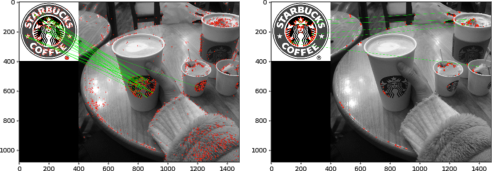
\includegraphics[width=0.5\textwidth]{sosanh.pdf} \\
\textbf{Figure 5. Matching results on Starbucks logo: SIFT-FLANN (left) and ORB-FLANN (right)}
\end{center}
\par
Considering the time-accuracy trade-off and the results from experiments, SIFT-FLANN is chosen as the base method for the improving methods. The average accuracy of SIFT-FLANN is 60.56\%.\par

\subsection{Generate keypoints by uniform sampling and distribute them over the entire logo}
Because of the shape of sample logos, we apply disk distribution on Pepsi logo and rectangle distribution on the others. As mentioned in section III, we choose to distribute random keypoints with radius 5. On the train image, keypoints are distributed only at the center for saliency detection purpose.\par
\begin{center}
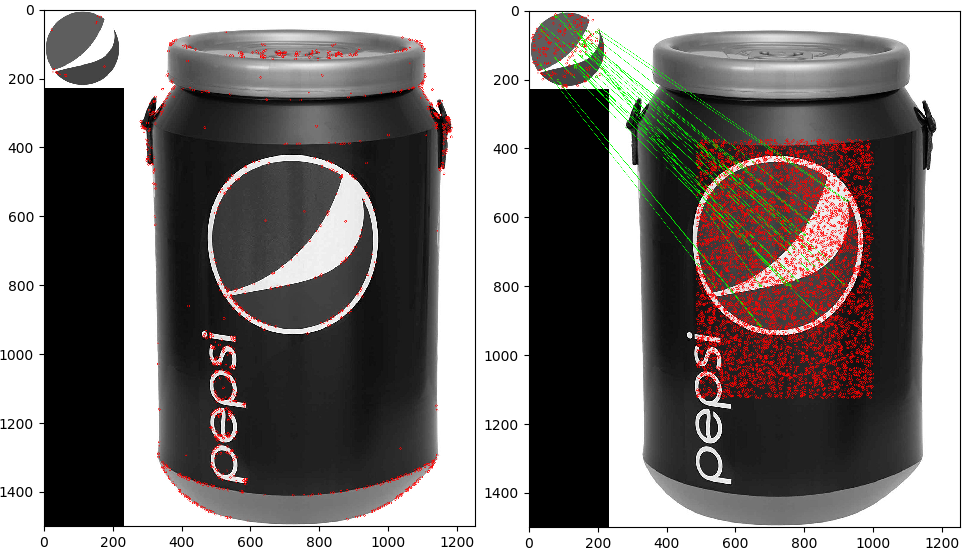
\includegraphics[width=0.5\textwidth]{sosanh0_200.png} \\
\textbf{Figure 6. Matching results on Pepsi logo:\\ SIFT-FLANN (left),\\ Uniform sampling with kp=200 (right)}
\end{center}
\par
Initially, we choose to distribute 200 keypoints (kp=200) on the query image (sample logo). Figure 6 illustrates a result on Pepsi logo: there are no matches in SIFT-FLANN combination, while the uniform sampling method performs well. Then when we generate more keypoints, the number of good matches increase, but the serious problem is the number of false matches also increase significantly. Figure 7 illustrates this point with kp=500 and kp=700, which false matches start to appear. The matches go outside the region of the logo. The reason is that we "force" the keypoints to lie randomly without using suitable detectors, they may lie on the regions that have similar features. Moreover, the case when the background has features similar to the sample logo also creates more noises.  \par
%\setkeys{Gin}{draft}

%\setkeys{Gin}{draft}
\begin{center}
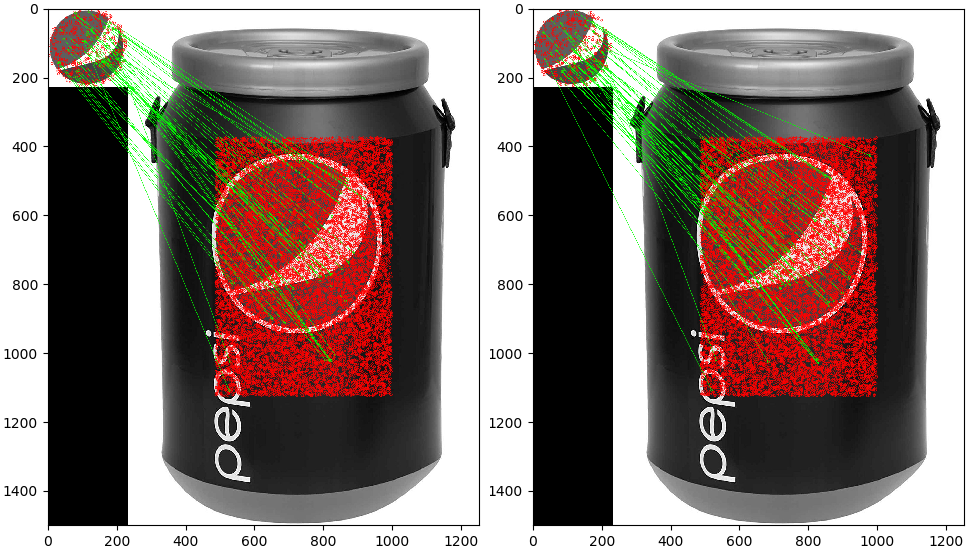
\includegraphics[width=0.5\textwidth]{sosanh500_700.png} \\
\textbf{Figure 7. Matching results on Pepsi logo:\\ Uniform sampling with kp=500 (left), kp=700 (right)}
\end{center}
\begin{center}
\begin{tabular}{|l|c|}
\hline
Logos & Accuracy\\ \hline
Vinamilk & 93.33\% \\ \hline
McDonald & 0.00\% \\ \hline
Pepsi & 29.41\% \\ \hline
Heineken & 83.33\% \\ \hline
Sprite & 26.92\% \\ \hline
Coca-Cola & 90.32\% \\ \hline
Starbucks & 100.00\% \\ \hline
Baskin Robbins & 90.48\% \\ \hline 
\end{tabular}
\\
\end{center}
\begin{center}
\textbf{Table 3. Results of the proposed method based on uniform sampling with kp=200}
\end{center}
\par
Table 3 shows the accuracy of each logo. The improvement in accuracy shows clearly in Pepsi and Hieneken cases: Pepsi increases from 0.00\% to 29.41\%, and Heineken increases about 13.33\% compared to SIFT-FLANN. McDonald still observes 0.00\% in accuracy. McDonald logo is simple, almost all of the keypoints lie in the regions that do not have characteristic features. Sprite and Starbucks do not show any improvements. The average running time of each image is 0.89s - about 2.3 times longer than SIFT-FLANN. The time is lengthened because of the distributing keypoints process. The average accuracy is 65.56\%.\par
To prevent the case of keypoints lying on similar regions, we decide to distribute them on the edges of the sample logo.
\subsection{Distribute keypoints on edges of the logo}
To test the effectiveness in eliminating false matches of this approach, we pick three logos that have low results in the previous experiment, which are McDonald, Pepsi and Sprite. We also choose Heineken and Coca-Cola to see whether this approach improves their accuracies. \par
\begin{center}
\begin{tabular}{|l|c|}
\hline
Logos & Accuracy\\ \hline
McDonald & 0.00\% \\ \hline
Pepsi & 0.00\% \\ \hline
Heineken & 46.67\% \\ \hline
Sprite & 0.00\% \\ \hline
Coca-Cola & 90.32\% \\ \hline
\end{tabular}
\\
\end{center}
\begin{center}
\textbf{Table 4. Results of uniform sampling on edges with kp=200}
\end{center}

\begin{center}
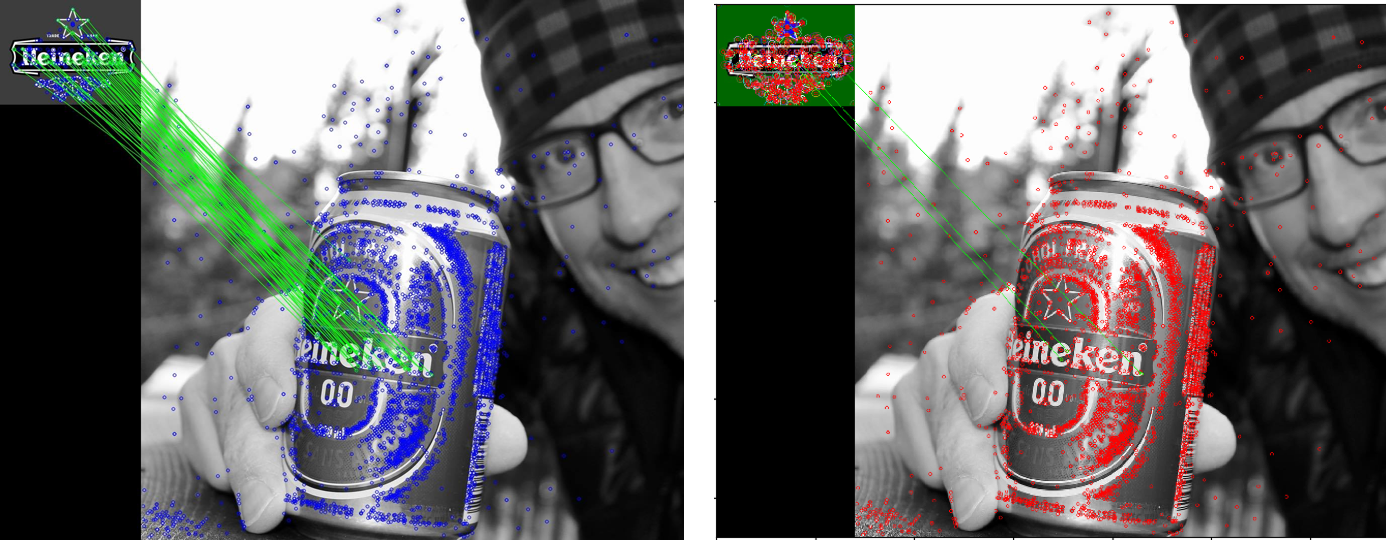
\includegraphics[width=0.5\textwidth]{sosanhheneken.png} \\
\textbf{Figure 8. Matchings results on Heineken logo:\\ SIFT-FLANN (left) and SIFT-FLANN with additional keypoints scattering on edge of the sample logo (right)}
\end{center}
\par
Surprisingly, the result is not better than the uniform sampling method as expected. In Table 4, the accuracy of Sprite decreases from 27.00\% to 0.00\%. Through experiment, each logo has the number of matching images shrinking progressively even though the running time is rising. The increase of average running time, which is 0.95s in this approach, is compensated for navigating the edge of logos and scattering keypoints on those edges. However, we notice that the false matchings between two images sink significantly. This decrease gives the assumption that the uniform-sampling-on-edge method helps decrease false matchings and, therefore, increases the quality of keypoint-matching method.\par
In Figure 8, the original SIFT-FLANN method gives the result with many false matchings. While, the SIFT-FLANN method combing with scattering keypoints on edge has all correct matchings although there are only four matchings.\par
\begin{center}
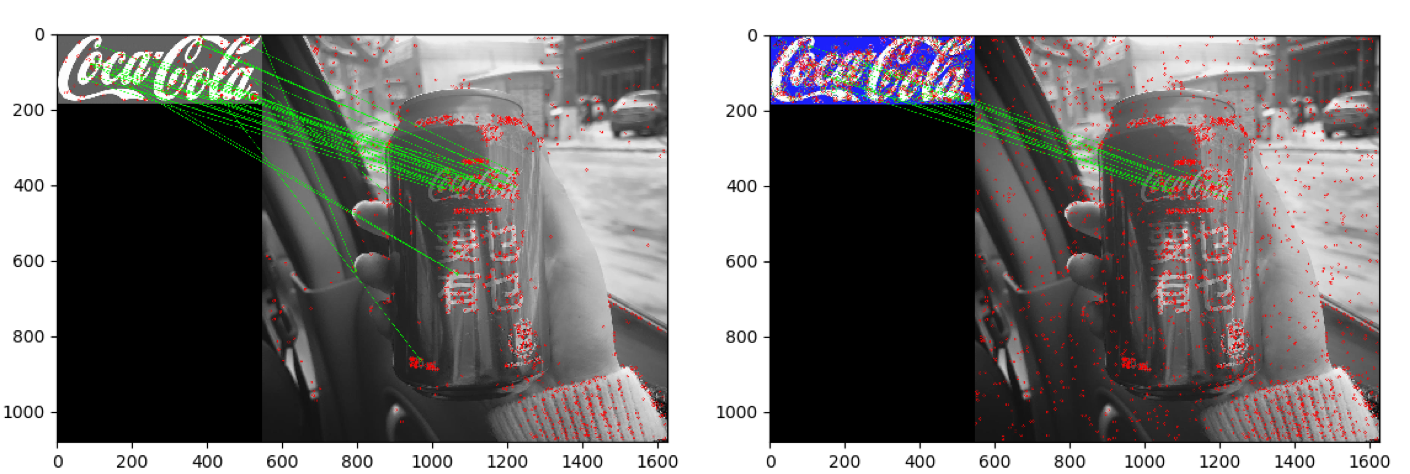
\includegraphics[width=0.5\textwidth]{sosancocacola.png} \\
\textbf{Figure 9. Matchings results on Coca-Cola logo:\\ SIFT-FLANN (left) and SIFT-FLANN with additional keypoints scattering on edge of the sample logo (right)}
\end{center}
\par
Logo of Coca-Cola is also used for testing with the proposed method. The quality of matchings is increased gradually although the running time is longer than 7.5 seconds compare to the original method SIFT-FLANN. In Figure 9, the false matchings which appears in the left picture of Coca-Cola logo are eliminated in the right picture.\par
\section{CONCLUSIONS \& FUTURE WORK}
We presented an improvement of traditional feature matching method, which inherits from uniform sampling. Our experiments demonstrate that the accuracy increases 5.00\% (from 60.56\% of original SIFT-FLANN to 65.56\% of the proposed method) on the combined dataset. Moreover, the approach of scattering keypoints on the logo edges also be proved to decrease noise matchings.\par
However, the problem of having few keypoints in logos still remains after a considerable effort to improve. The future work is to find an alternative method which is necessary to deal with few-featured logos. Our direction is to combine machine learning method into the process. With the goal to help the companies in conducting customer experiences through the massive amount of photos in social networks, it is our work to adapt the method into real-time applications. For example, by mobiles real-time applications, which the customers can use to detect the brands logos, offline-to-online commerce is developed.
\bibliographystyle{unsrt} % sua thanh unsrt de theo thu tu
\bibliography{refs} % Entries are in the "refs.bib" file

\end{document}
